\documentclass[12pt]{article}
\usepackage{graphicx}
\usepackage{caption}
\usepackage{geometry}
\geometry{margin=1in}
\usepackage{titlesec}
\titleformat{\section}{\normalfont\Large\bfseries}{\thesection.}{1em}{}

\title{PTL-X Trauma Simulation Report}
\author{Breezon Brown}
\date{}

\begin{document}

\maketitle

\section*{System Description}
PTL-X (Recursive Time Distortion Engine) models trauma-induced time distortion using recursive memory bifurcation and synthetic EEG echo dynamics. This report visualizes 10 unique waveform cases simulating escalating trauma signatures, from stable rhythm to recursive chaos.

\section*{Simulation Suite Summary}
\begin{itemize}
  \item \textbf{Case 1 (Normal Sine)}: Control baseline. Healthy memory rhythm.
  \item \textbf{Case 2 (Exponential Decay)}: PTSD latency onset. Trauma absorption phase.
  \item \textbf{Case 3 (Bifurcation)}: Memory collapse zone. Recursive instability.
  \item \textbf{Case 4 (Tan-Sine Conflict)}: Fragmented narrative trauma. Cognitive dissonance loop.
  \item \textbf{Case 5 (Flatline)}: Emotional numbness. Recursion death.
  \item \textbf{Case 6 (Logistic Chaos)}: Unstable memory integration. Edge of disorder.
  \item \textbf{Case 7 (Gaussian Noise)}: Panic state. Acute disarray.
  \item \textbf{Case 8 (Biased Noise)}: Depression signal. Emotional skew.
  \item \textbf{Case 9 (Low-Freq + Noise)}: Rumination loop. Blurred echo.
  \item \textbf{Case 10 (High-Freq Chaos)}: Cognitive flood. Signal overload.
\end{itemize}

\newpage

\section*{Case 1: Normal Sine}
\begin{center}
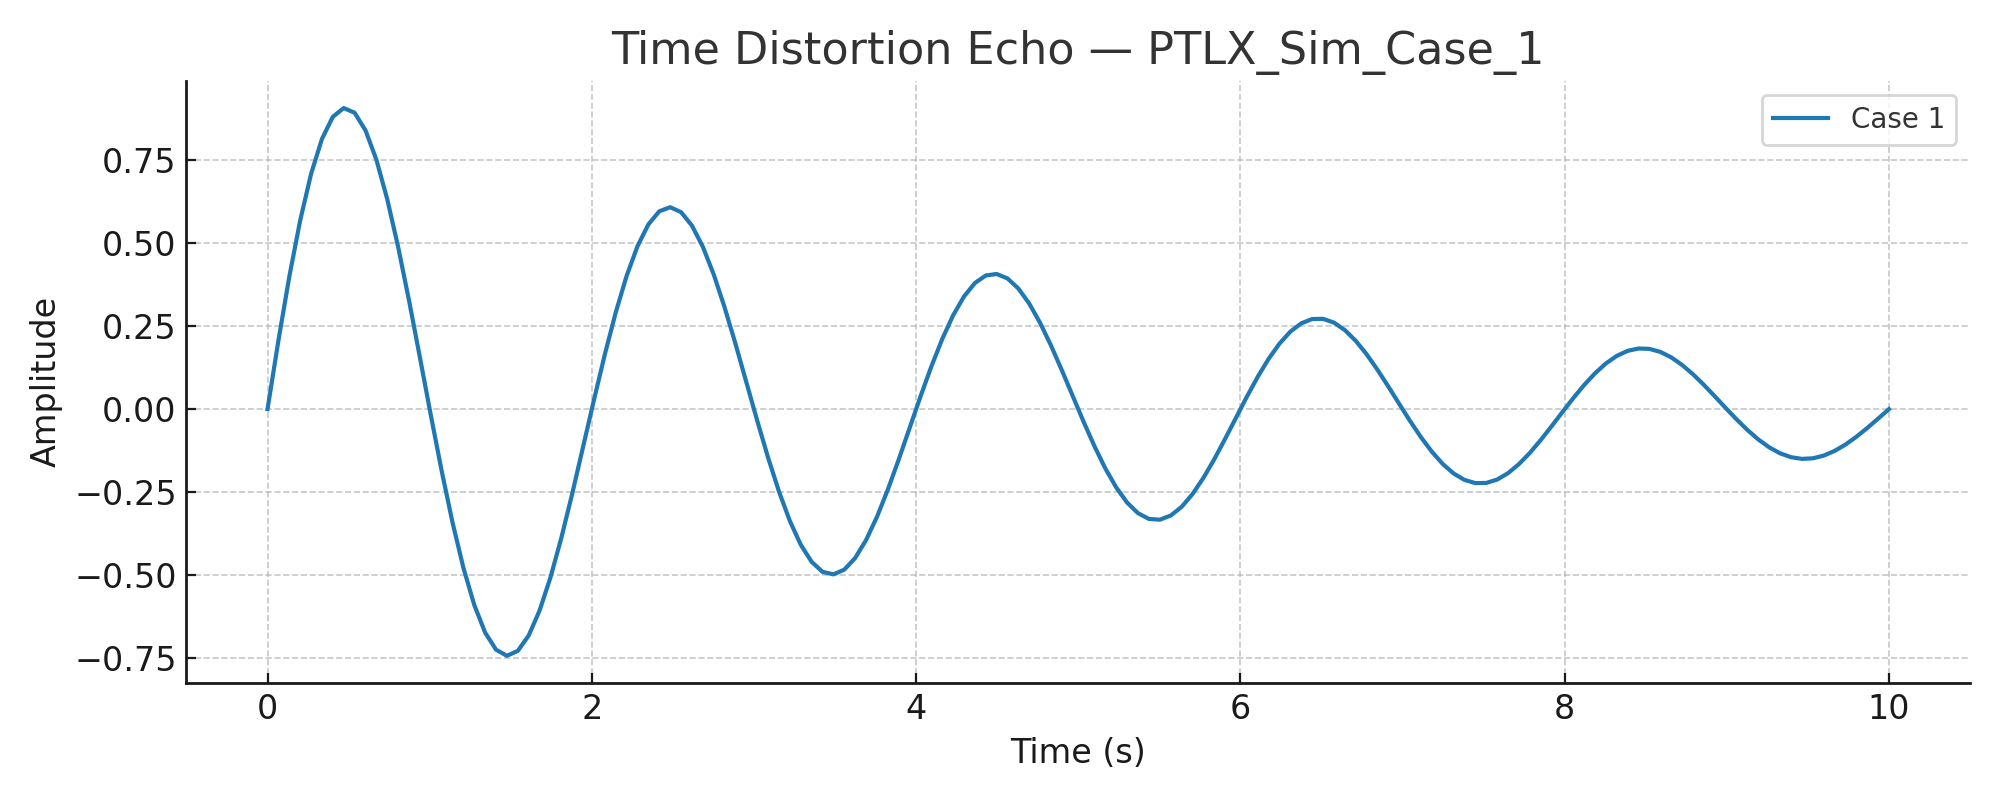
\includegraphics[width=0.95\linewidth]{PTLX_Sim_Case_1.png}
\end{center}
\textbf{Description}: Stable sinusoidal wave \\

\textbf{Clinical Meaning}: Healthy memory rhythm. No trauma detected.

\newpage

\section*{Case 2: Exponential Decay}
\begin{center}
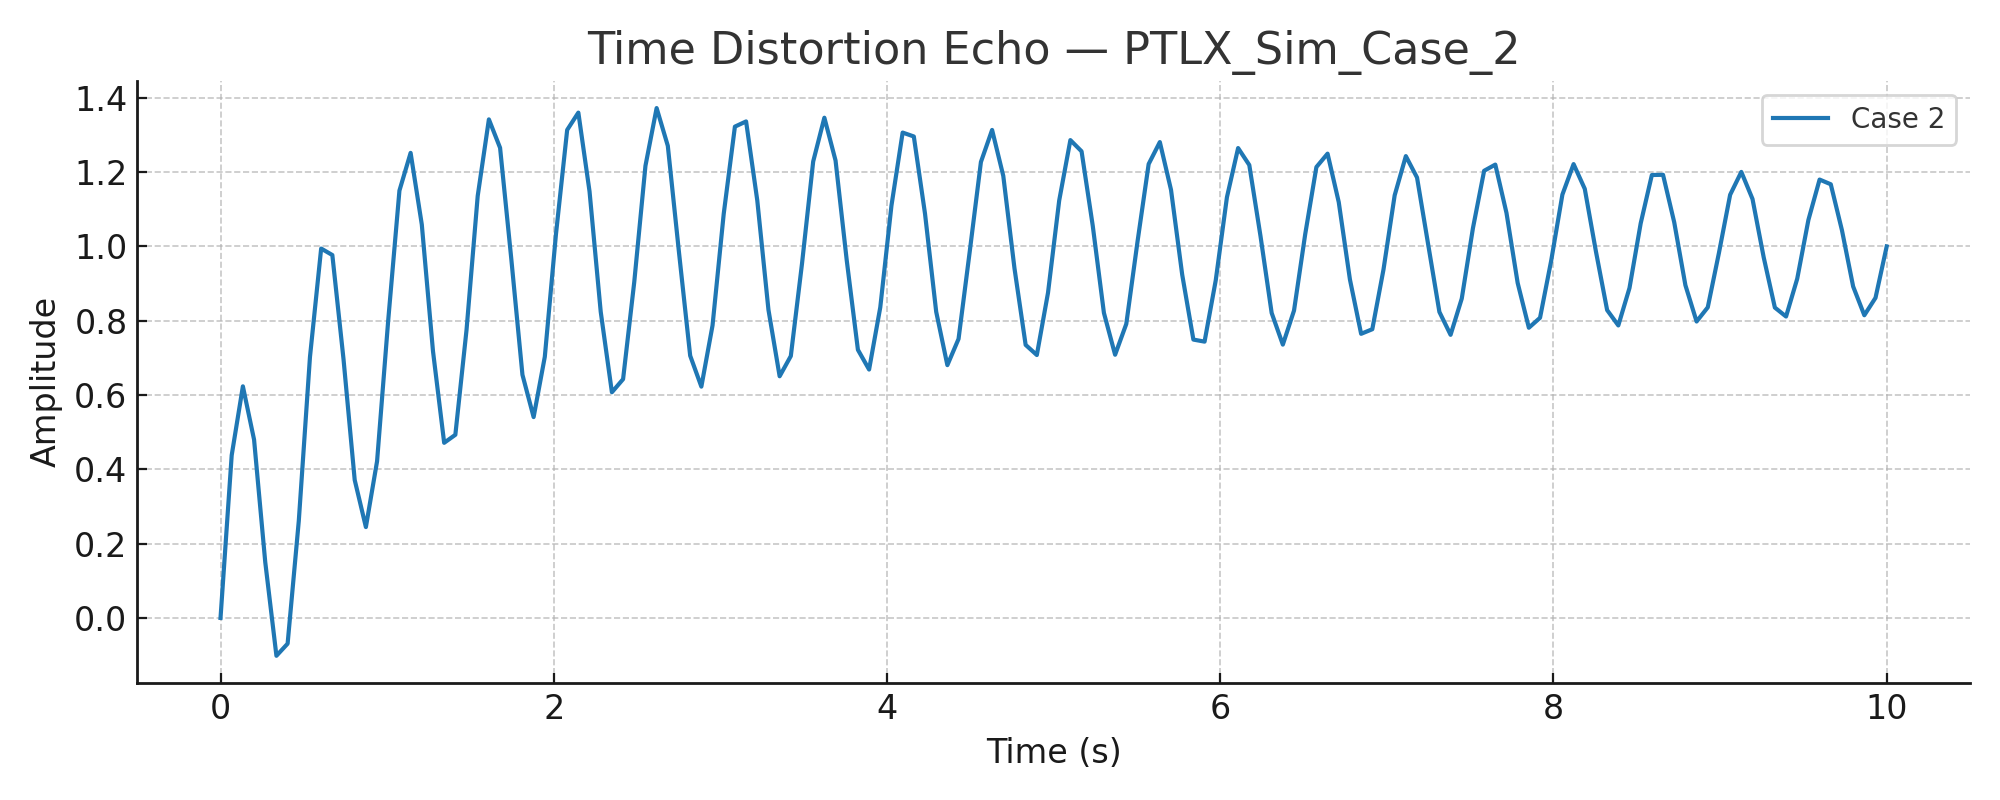
\includegraphics[width=0.95\linewidth]{PTLX_Sim_Case_2.png}
\end{center}
\textbf{Description}: Declining energy curve \\

\textbf{Clinical Meaning}: Latent trauma with memory suppression dynamics.

\newpage

\section*{Case 3: Bifurcation}
\begin{center}
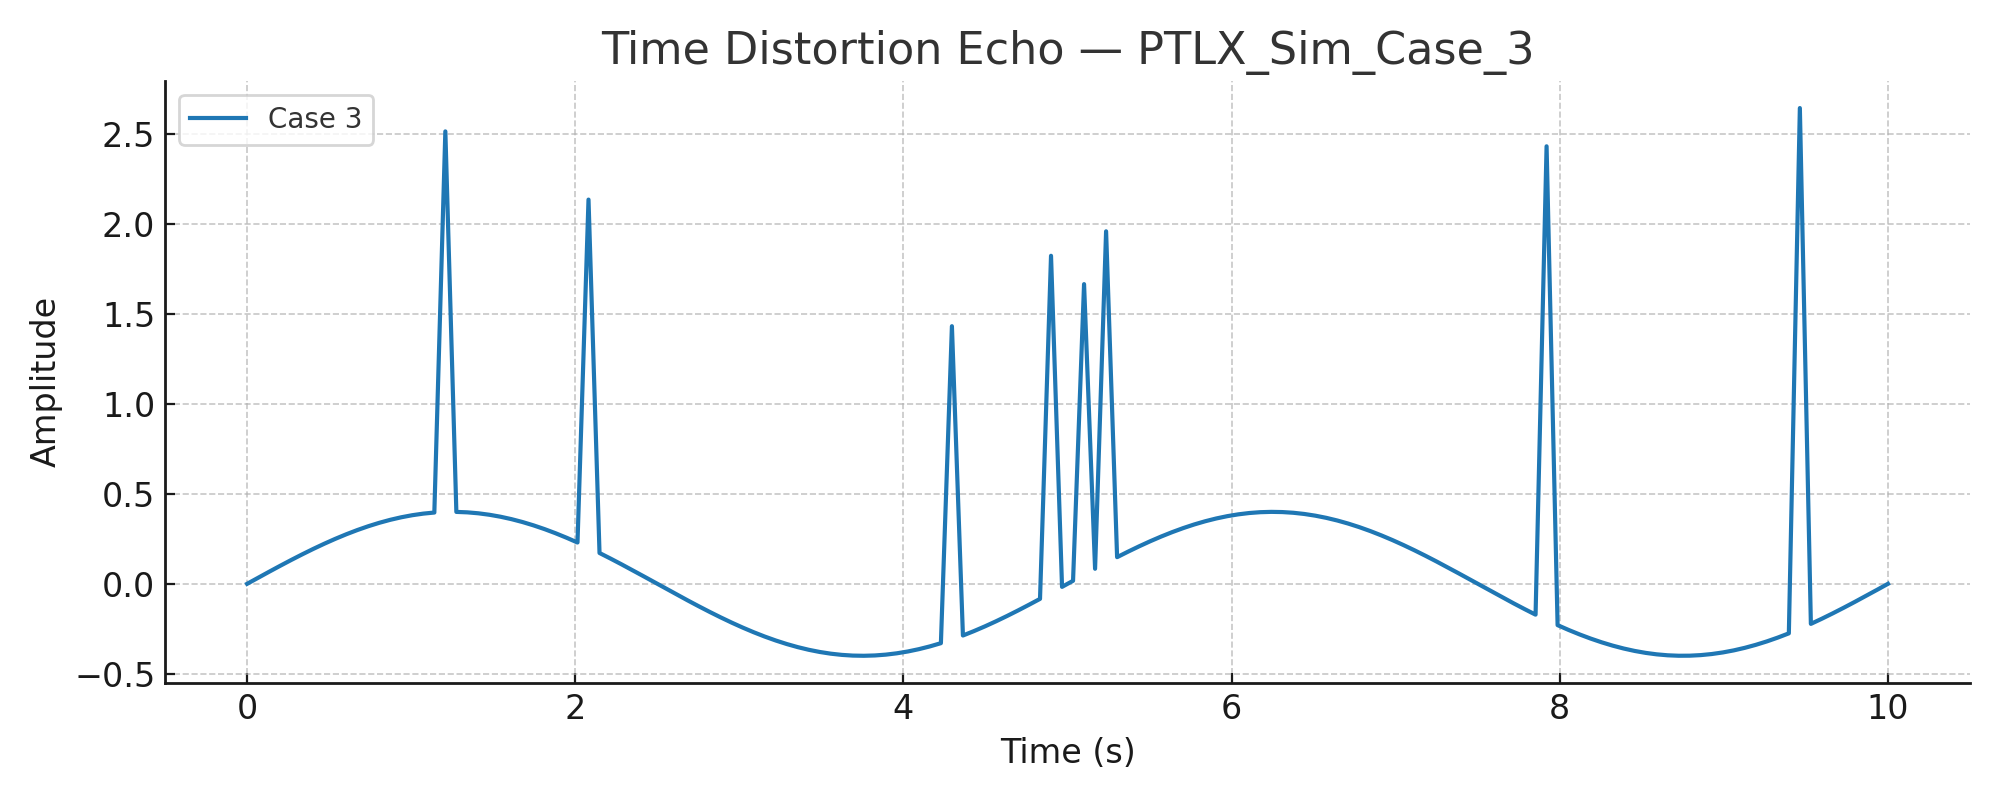
\includegraphics[width=0.95\linewidth]{PTLX_Sim_Case_3.png}
\end{center}
\textbf{Description}: Split-phase oscillation \\

\textbf{Clinical Meaning}: Onset of recursive trauma loop. Time fracture point.

\newpage

\section*{Case 4: Tan-Sine Conflict}
\begin{center}
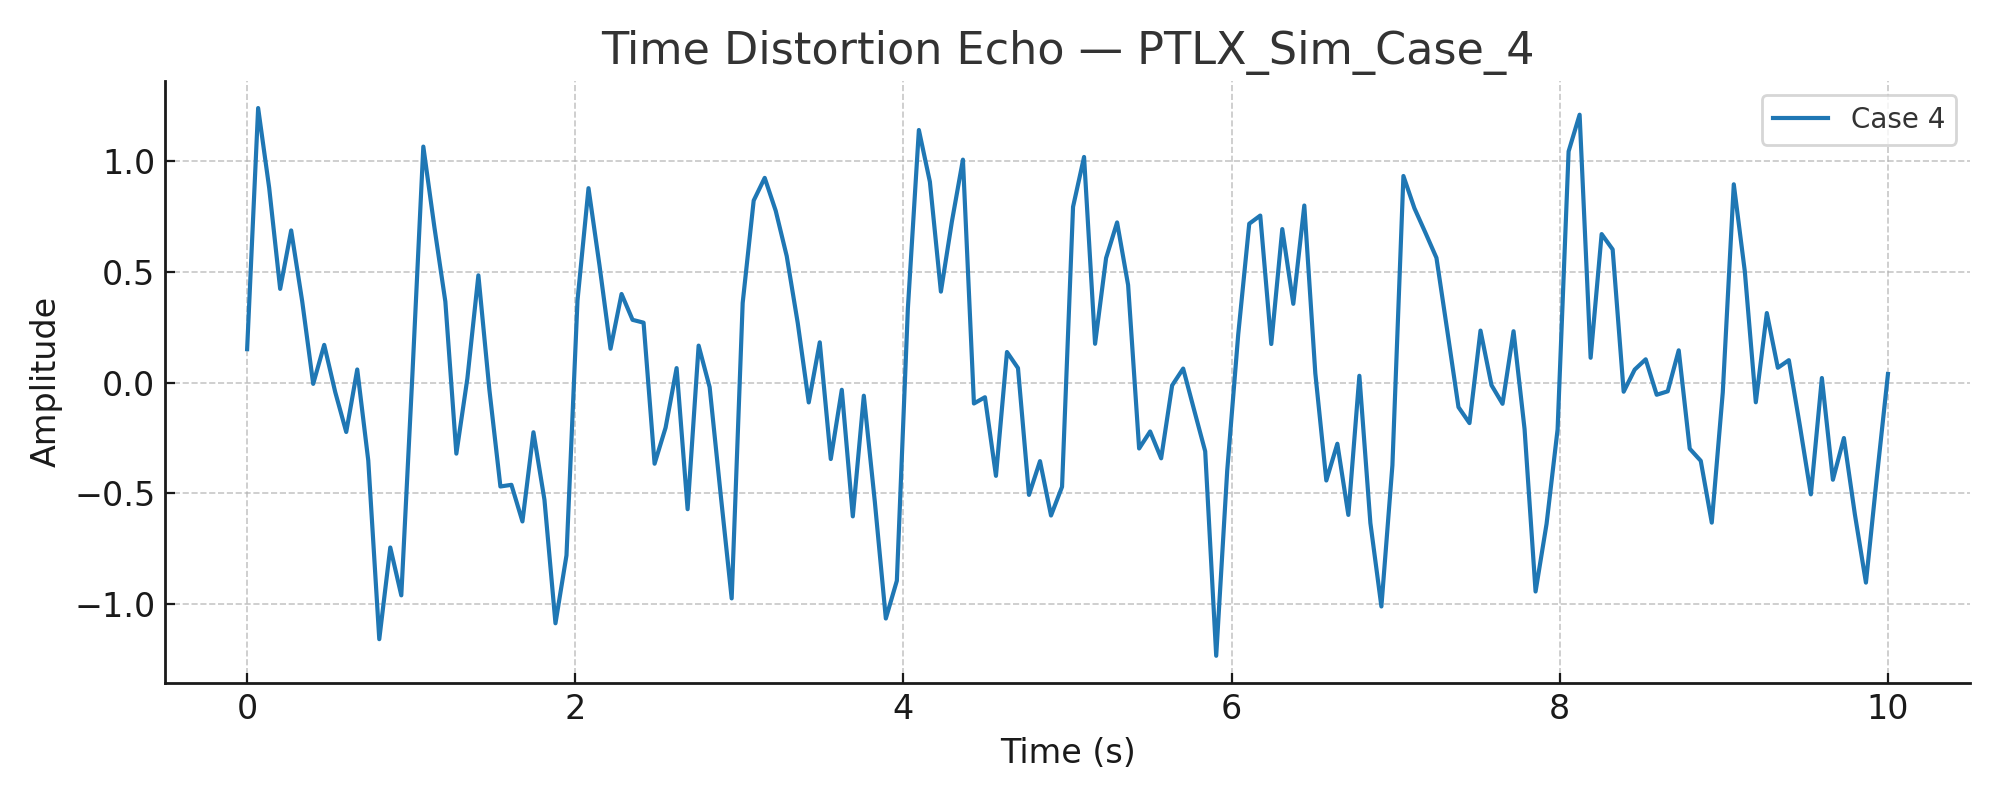
\includegraphics[width=0.95\linewidth]{PTLX_Sim_Case_4.png}
\end{center}
\textbf{Description}: Cognitive interference \\

\textbf{Clinical Meaning}: Competing memory signals; dissociative trauma.

\newpage

\section*{Case 5: Flatline}
\begin{center}
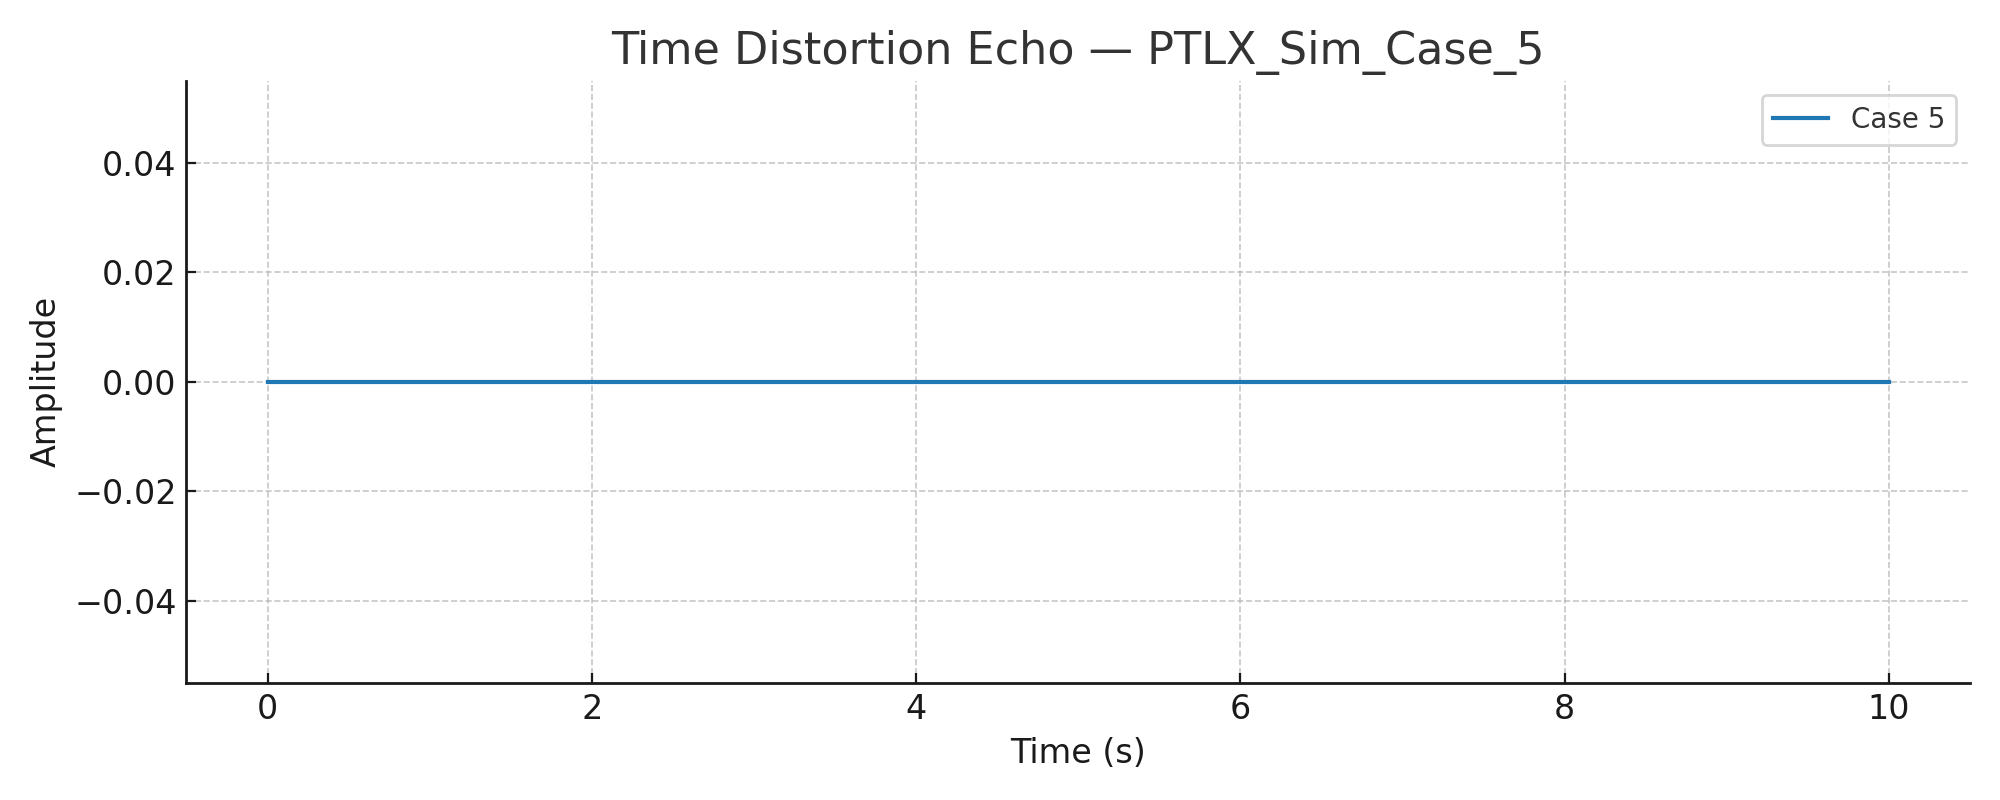
\includegraphics[width=0.95\linewidth]{PTLX_Sim_Case_5.png}
\end{center}
\textbf{Description}: No activity \\

\textbf{Clinical Meaning}: Emotional blackout. Trauma-induced void state.

\newpage

\section*{Case 6: Logistic Chaos}
\begin{center}
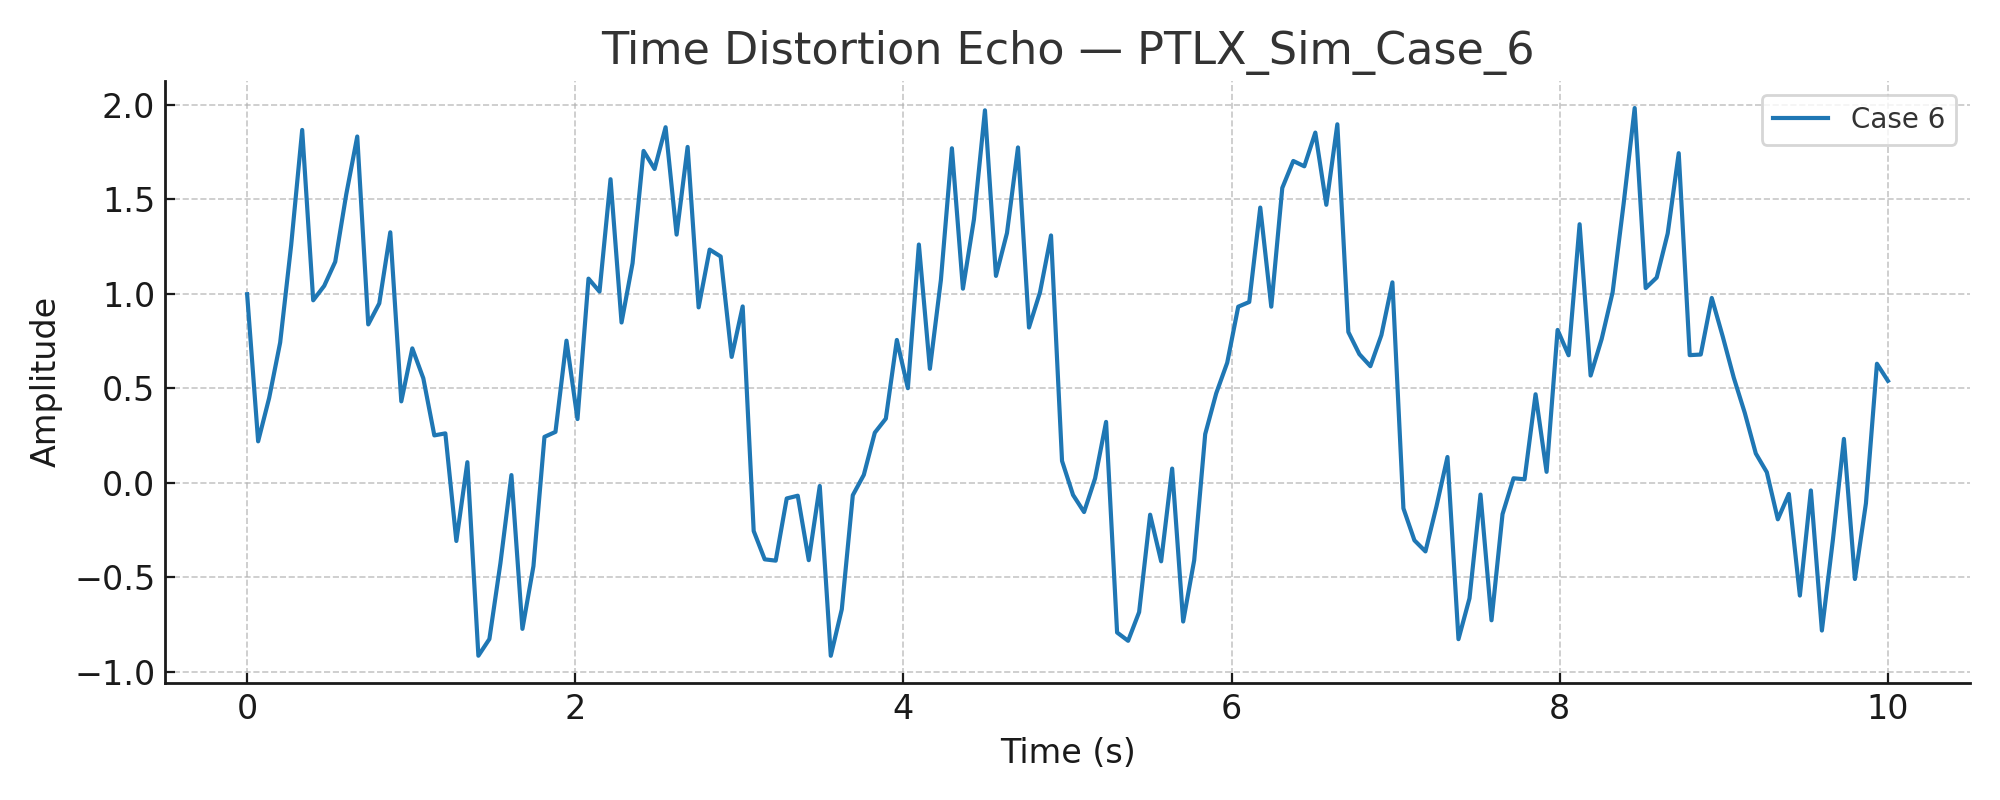
\includegraphics[width=0.95\linewidth]{PTLX_Sim_Case_6.png}
\end{center}
\textbf{Description}: Nonlinear recursion \\

\textbf{Clinical Meaning}: Disorganized trauma processing. Unstable integration.

\newpage

\section*{Case 7: Gaussian Noise}
\begin{center}
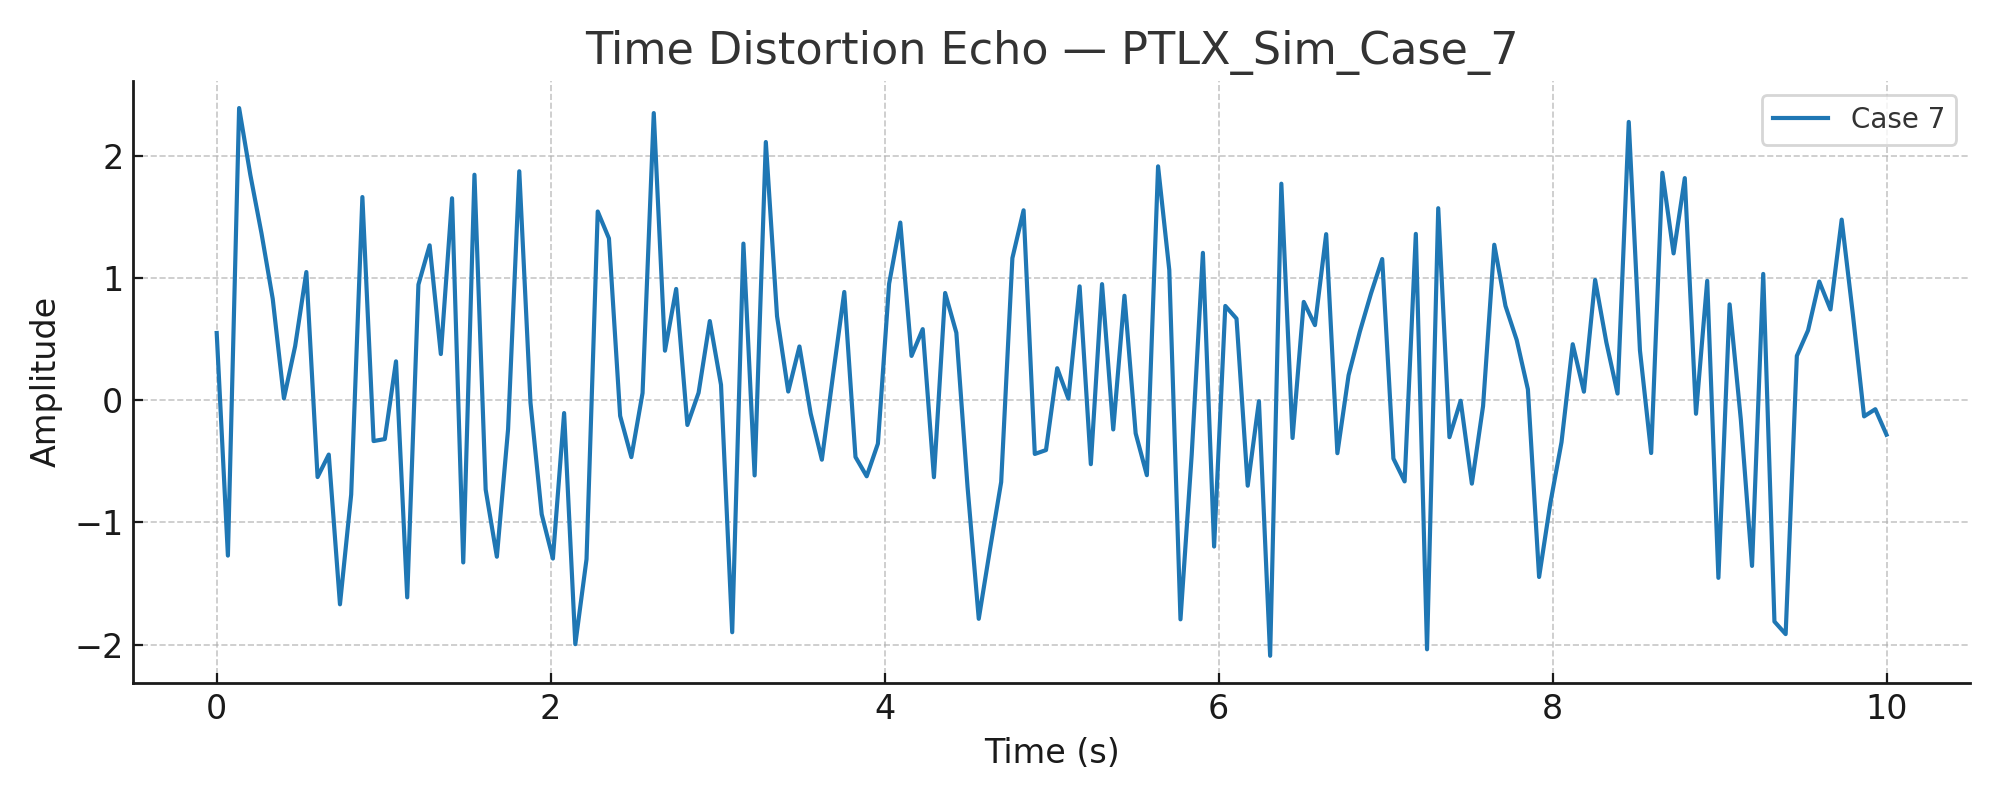
\includegraphics[width=0.95\linewidth]{PTLX_Sim_Case_7.png}
\end{center}
\textbf{Description}: Random spikes \\

\textbf{Clinical Meaning}: Panic disorder wave pattern. High entropy state.

\newpage

\section*{Case 8: Biased Noise}
\begin{center}
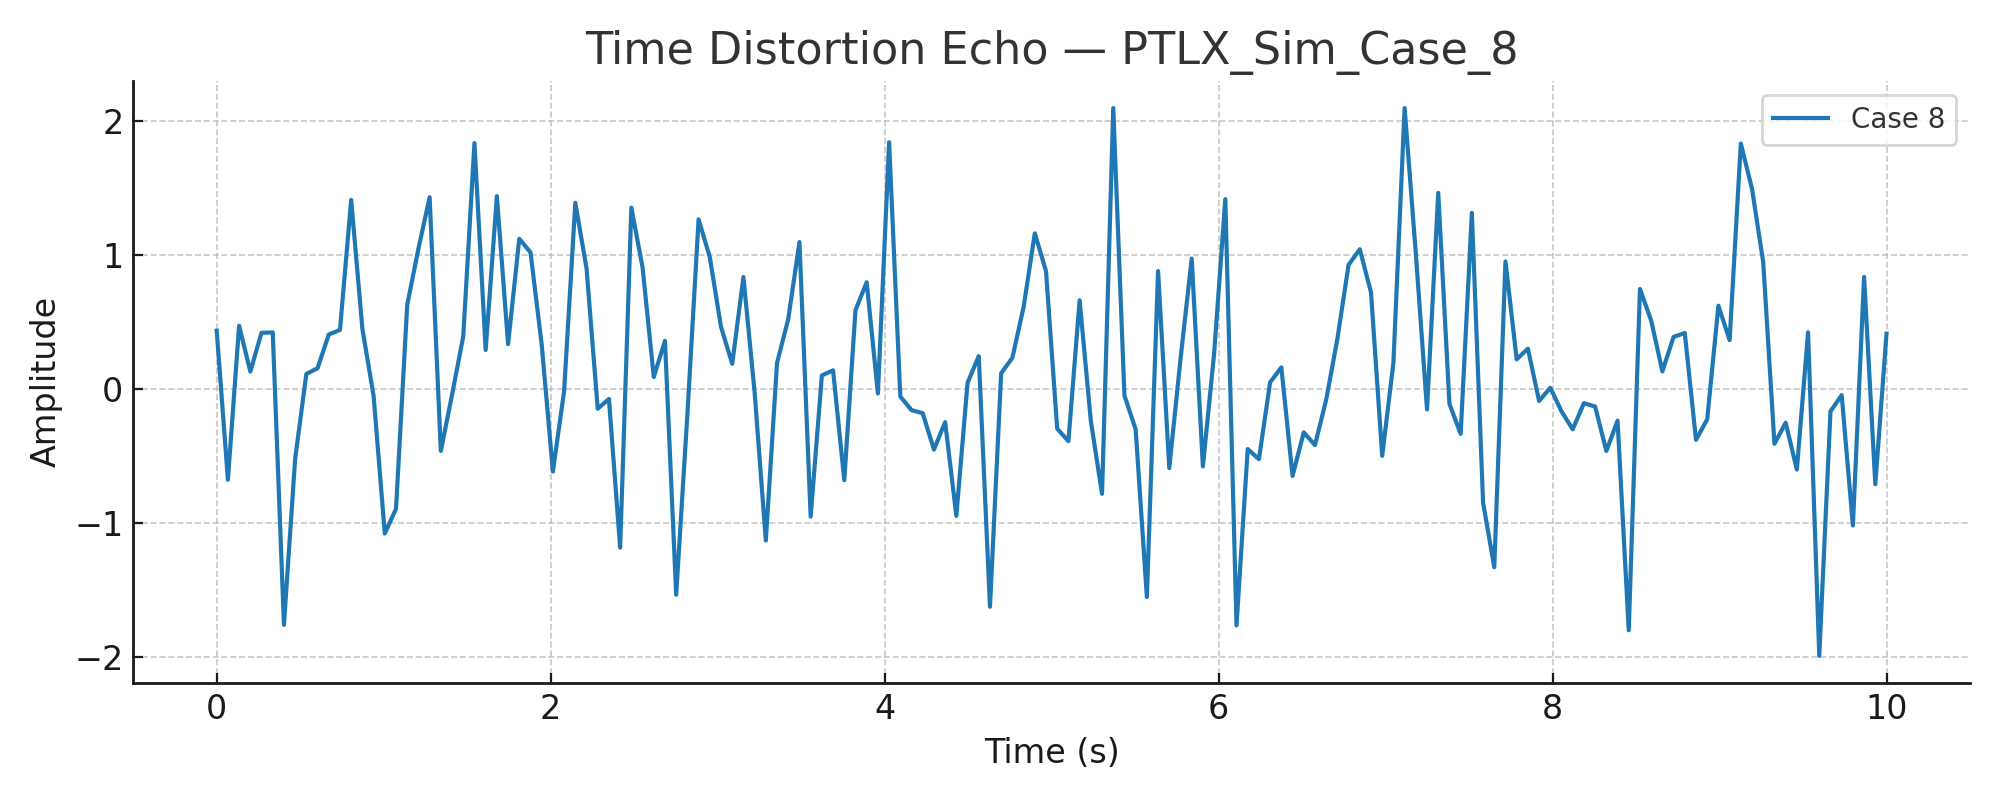
\includegraphics[width=0.95\linewidth]{PTLX_Sim_Case_8.png}
\end{center}
\textbf{Description}: Low-energy noise with slope \\

\textbf{Clinical Meaning}: Melancholy/depression. Downshifted recursion.

\newpage

\section*{Case 9: Low-Freq + Noise}
\begin{center}
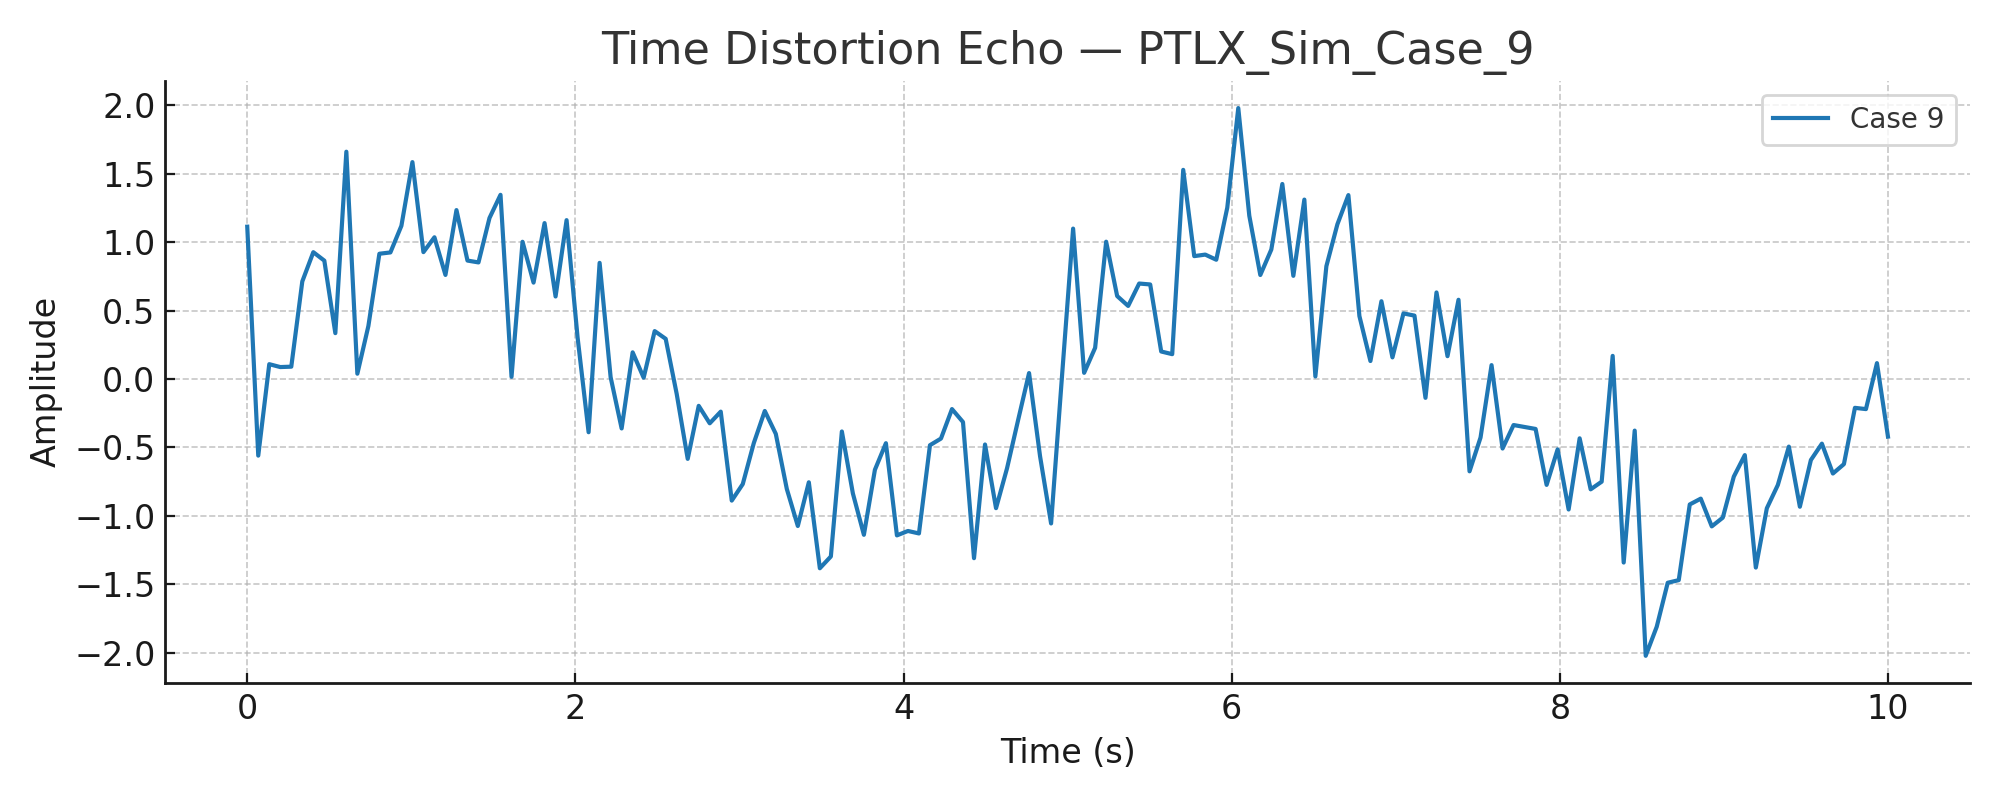
\includegraphics[width=0.95\linewidth]{PTLX_Sim_Case_9.png}
\end{center}
\textbf{Description}: Rumination pattern \\

\textbf{Clinical Meaning}: Partial memory collapse with blurred loops.

\newpage

\section*{Case 10: High-Freq Chaos}
\begin{center}
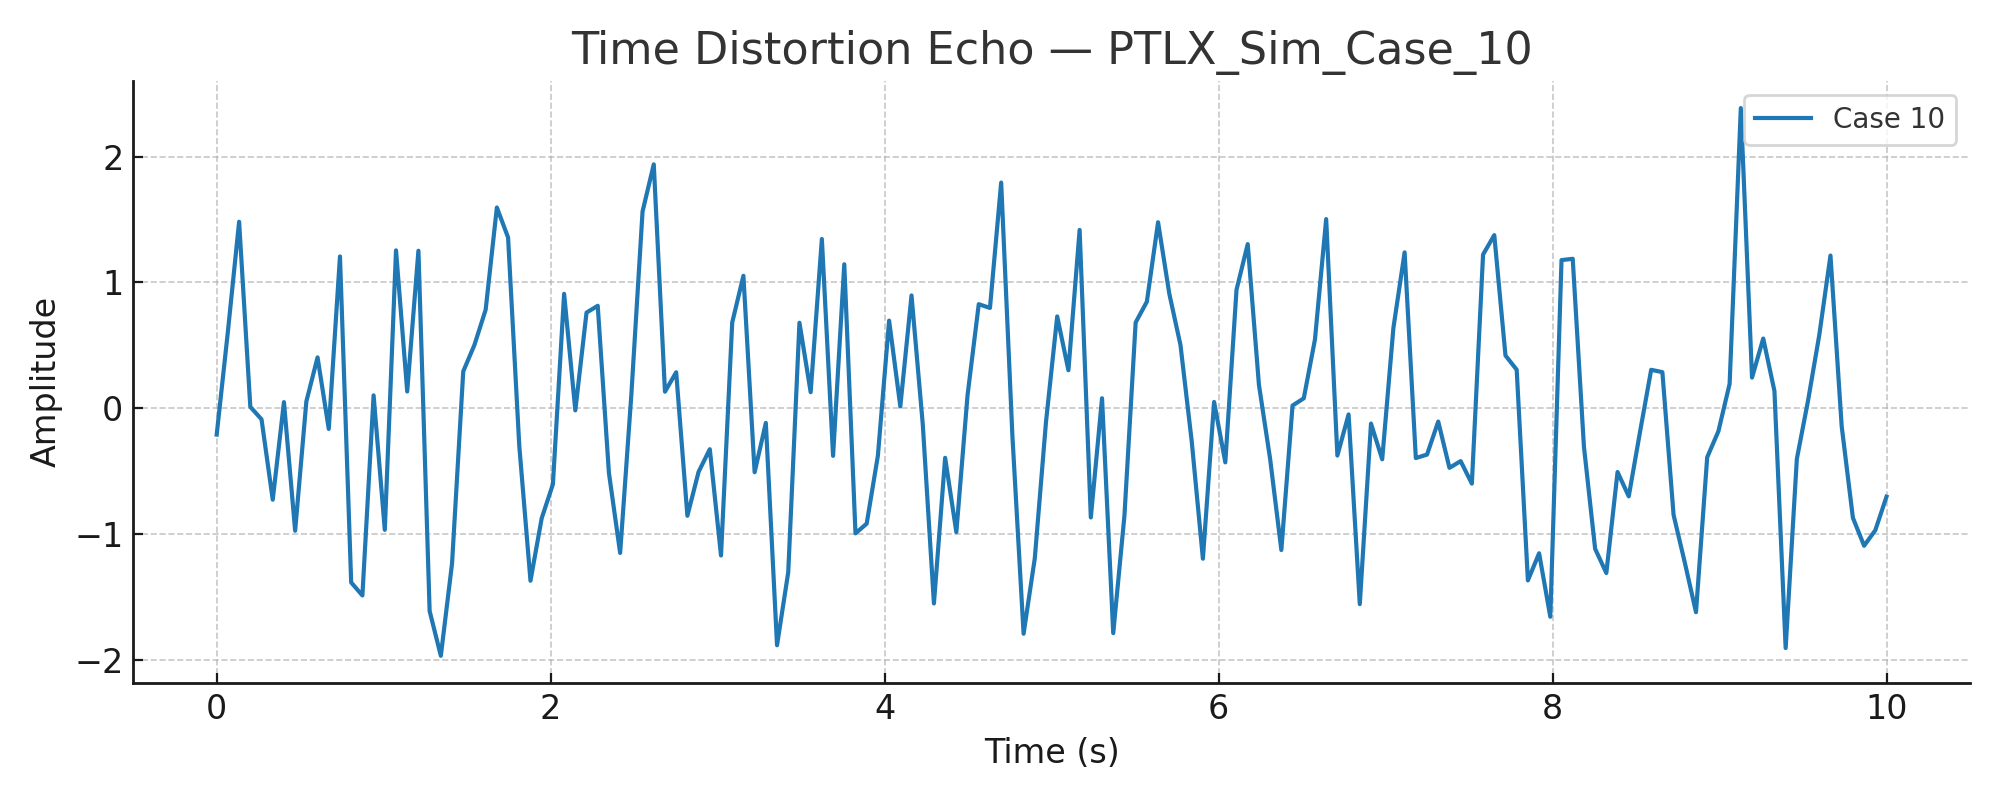
\includegraphics[width=0.95\linewidth]{PTLX_Sim_Case_10.png}
\end{center}
\textbf{Description}: Overload state \\

\textbf{Clinical Meaning}: Extreme trauma echo. System breakdown imminent.

\newpage
\end{document}